%!TEX root = ../../Main.tex
\graphicspath{{Chapters/Struktur/}}
%-------------------------------------------------------------------------------

\section{TFT Display Module}
TFT Display modulets primære opgave er både at fungere som visuel grænse flade til brugeren, samt at fungere som et slags kontrol modul for hele systemet. Kontrol modul forstået på den måde, at dette modul står for at hente data fra Color Sensor Modulet, og optælle den hentede information. Dette modul afsnit vil beskrive TFT Display modulets funktionalitet, samt overvejelser omkring analyse og design både hardware, softwaremæssigt. I dette afsnit vil kommunikationen mellem TFT Display modulet og resten af systemet også blive beskrevet. 

\subsection{Hardware}
I arkitekturfasen gik den første overvejelse på hvilket display vi skulle benytte som grænsefladen til brugeren. Vi ønskede et displayet som kunne vise farver og havde en nogenlunde opløsning for give en god visuel oplevelse for brugeren. Da vi først havde opsat kravene for vores display, var selve valget ikke særligt svært. I undervisningen har vi arbejdet med ”Graphic TFT Display”, dette display opfyldte vores ønskede krav angående opløsning samt muligheden for at vise farver. Derfor faldt valgt ret hurtigt på dette display, da det også spillede sammen med vores Arduino 2560. For at kunne påmontere ”Graphic TFT Display” på Arduino Mega 2560, har vi benyttet os af ”ITDB02 Arduino MEGA shield 2.0”. Databladet for dette shield er vedhæftet XX. I dette datablad er det også markeret hvilke porte ITDB02 shieldet der hører til bestemte indgange på displayet.

\subsection{Software}
I og med at dette moduls primære opgave er at være visuel grænseflade for brugeren, har langt det meste arbejde med dette modul lagt i softwaren. 
Hvis man kigger på Graphic TFT Display, kan den fungere i fire forskellige MCU-Interface modes, hvilket simpelt betyder, hvor stor en bus-interface man ønsker at arbejde med. Vi har valgt at arbejde med 16-bit bus-interface. 

\begin{figure}[H]
	\centering
	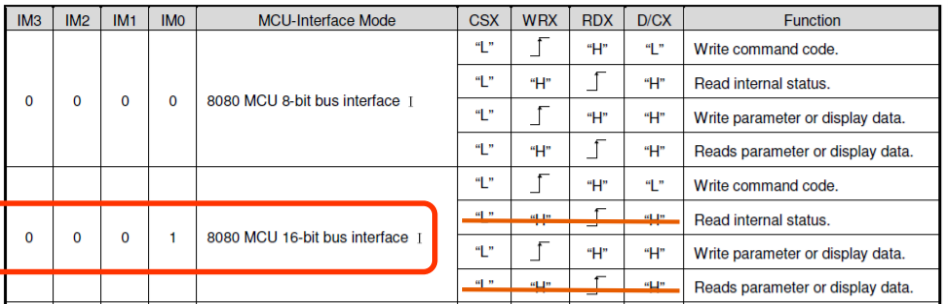
\includegraphics[width = 400pt]{Img/MCU-Interface_Mode.png}
	\caption{MCU-Interface Mode}
	\label{fig:MCU-Interface_Mode}
\end{figure}

I og med at vi udelukkende ønsker at skrive til vores display, vælger vi at ignorere læse kommandoerne og udelukkende fokusere på at skrive kommandoerne. Derfor er RDX altid sat høj.
Først implementerede vi WriteCommand i vores kode som ses på figur \autoref{fig:WriteCommand_Code} nedenfor

\begin{figure}[H]
	\centering
	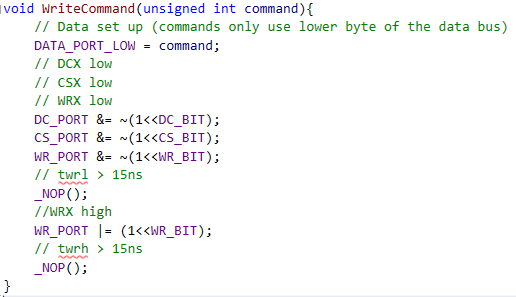
\includegraphics[width = 300pt]{Img/WriteCommand_Code.png}
	\caption{WriteCommand kode}
	\label{fig:WriteCommand_Code}
\end{figure}


Som det ses på figur \autoref{fig:MCU-Interface_Mode} fra databadet skal DCX og CSX sættes lavt, samt trigger kommandoen på WRX stigende flanke, derfor sættes WRX lav til at starte med. På figur \autoref{fig:Timedelays} nedenfor ses et skema over de tidsforsinkelser der opstår, ved forskellige operationer. Her ses det at når WRX sættes lav, opstår der en forsinkelse på min 15ns. Derfor er der indsat en NOP() funktion i koden, hvilket står for ”No Operation” som vil sige at programmet laver ingenting i en cyklus. Med en MCPU frekvens på 16Mhz svare det til 62,5ns. Herefter sættes WRX høj igen for at trigger kommandoen efterfulgt af endnu en NOP() funktion da der opstår samme forsinkelse når WRX sættes høj.

\begin{figure}[H]
	\centering
	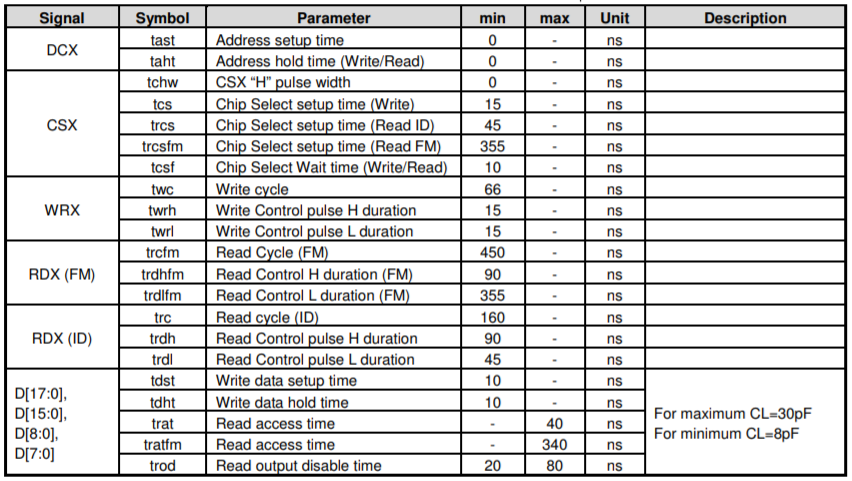
\includegraphics[width = 450pt]{Img/Timedelays.png}
	\caption{Tidsforsinkelser}
	\label{fig:Timedelays}
\end{figure}


Dernæst implementerede vi WriteData, som tilnærmelsesvis ligner WriteCommand bortset fra at DCX skal sættes høj i stedet for lav. Koden for WriteData ses nedenfor på figur \autoref{fig:WriteData_Code}. På samme måde som WriteCommand trigger WriteData på en voksende flanke på WRX, derfor sættes WRX først lav og dernæst høj, med indsat NOP() funktioner for at tage højde for tidsforsinkelser. 

\begin{figure}[H]
	\centering
	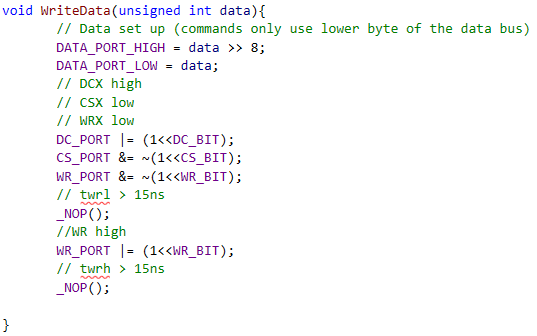
\includegraphics[width = 350pt]{Img/WriteData_Code.png}
	\caption{WriteData kode}
	\label{fig:WriteData_Code}
\end{figure}


I vores DisplayInit() som vi kalder en gang i koden til at Initialisere displayet, starter vi med at sætte vores Control Pins som output samt sætte dem høje. Dernæst bliver RST sat lav i 300ms, det skyldes at der i databladet på side 230 står minimum 120ms, så det er sat til 300ms for at være på den sikre side. Efter vi igen sætter RST igen bliver sat høj, skal vi igen vente 120ms før vi må kalde SleepOut Command, derfor indsætter et delay på 130ms. 

\begin{figure}[H]
	\centering
	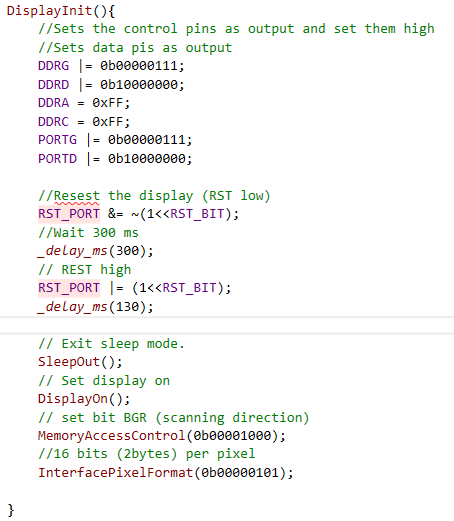
\includegraphics[width = 350pt]{Img/DisplayInit_Code.png}
	\caption{DisplayInit kode}
	\label{fig:DisplayInit_Code}
\end{figure}